\section{Análisis Experimental}

\begin{figure}
  \begin{center}
  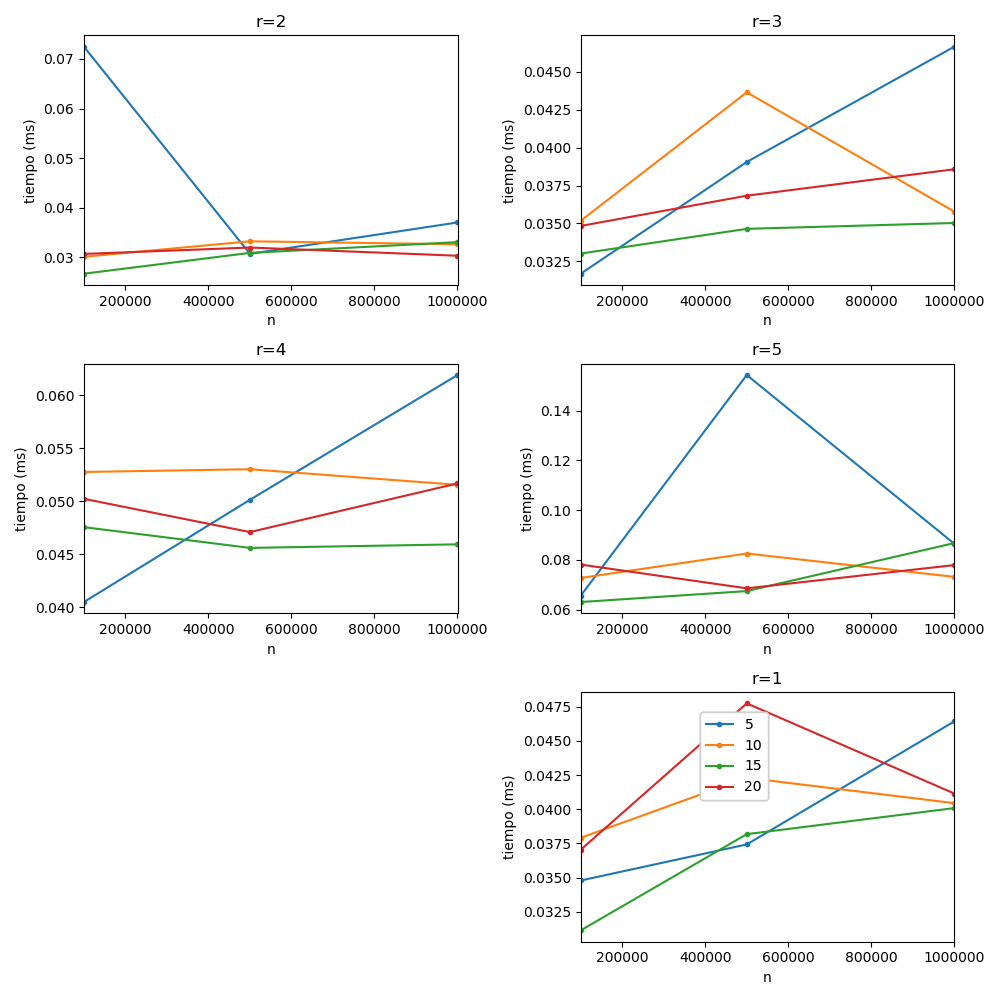
\includegraphics[width=.7\textwidth]{buscar_pos_n}
  \caption{Tiempo de búsqueda (positiva)
    según n, para distintos valores de r y k.}
  \label{fig:buscar-pos}
  \end{center}
\end{figure}


\begin{figure}
  \begin{center}
  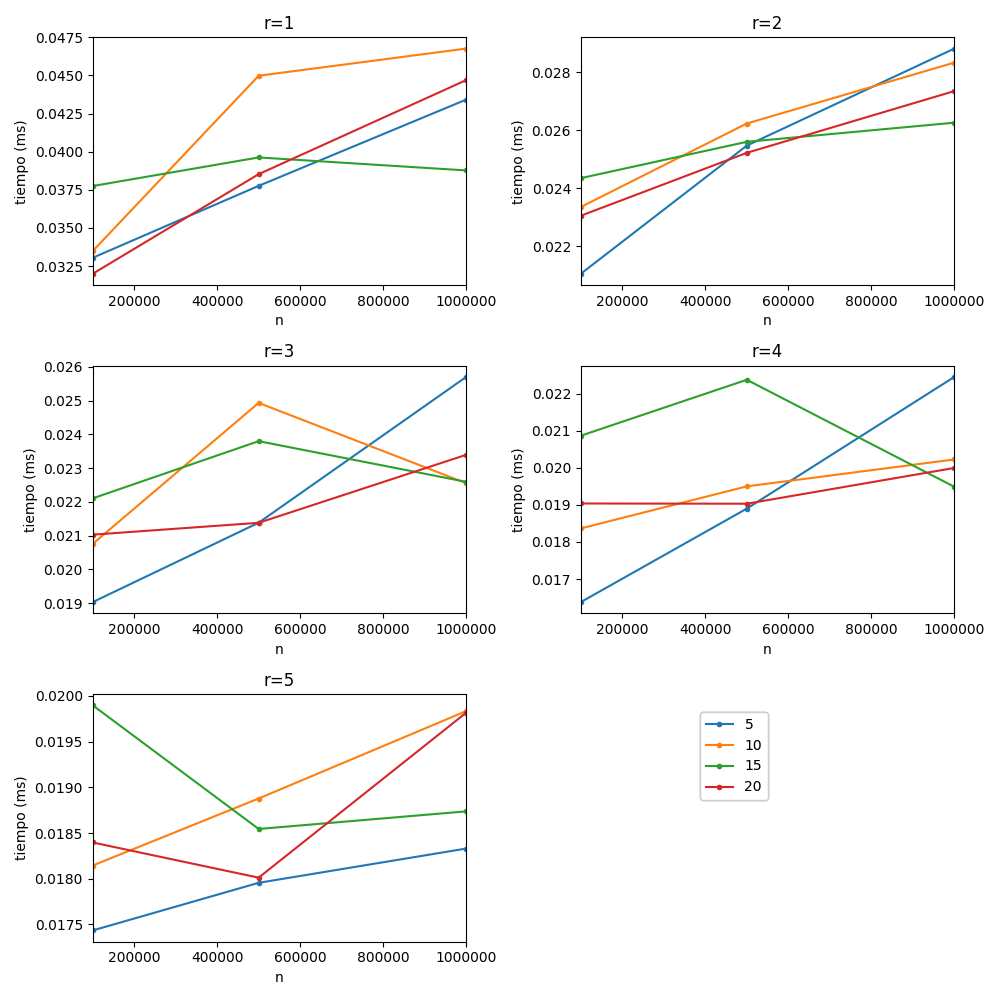
\includegraphics[width=.7\textwidth]{buscar_neg_n}
  \caption{Tiempo de búsqueda (negativa)
    según n, para distintos valores de r y k.}
  \label{fig:buscar-neg}
  \end{center}
\end{figure}

En las figuras \ref{fig:buscar-pos} y \ref{fig:buscar-neg} podemos
ver un crecimiento ligeramente cercano al logarítmico (que con tan solo 3
valores para \(n\)\footnote{Como se indica en la consigna} es dificil
distinguir).

La diferencia para distintos r (dado un k) se observa en la figura
\ref{fig:buscar}, y en todos los casos podemos observar que el árbol
con mayor r tiene un mejor rendimiento para las búsquedas tanto positivas como
negativas.

\begin{figure}
  \begin{center}
  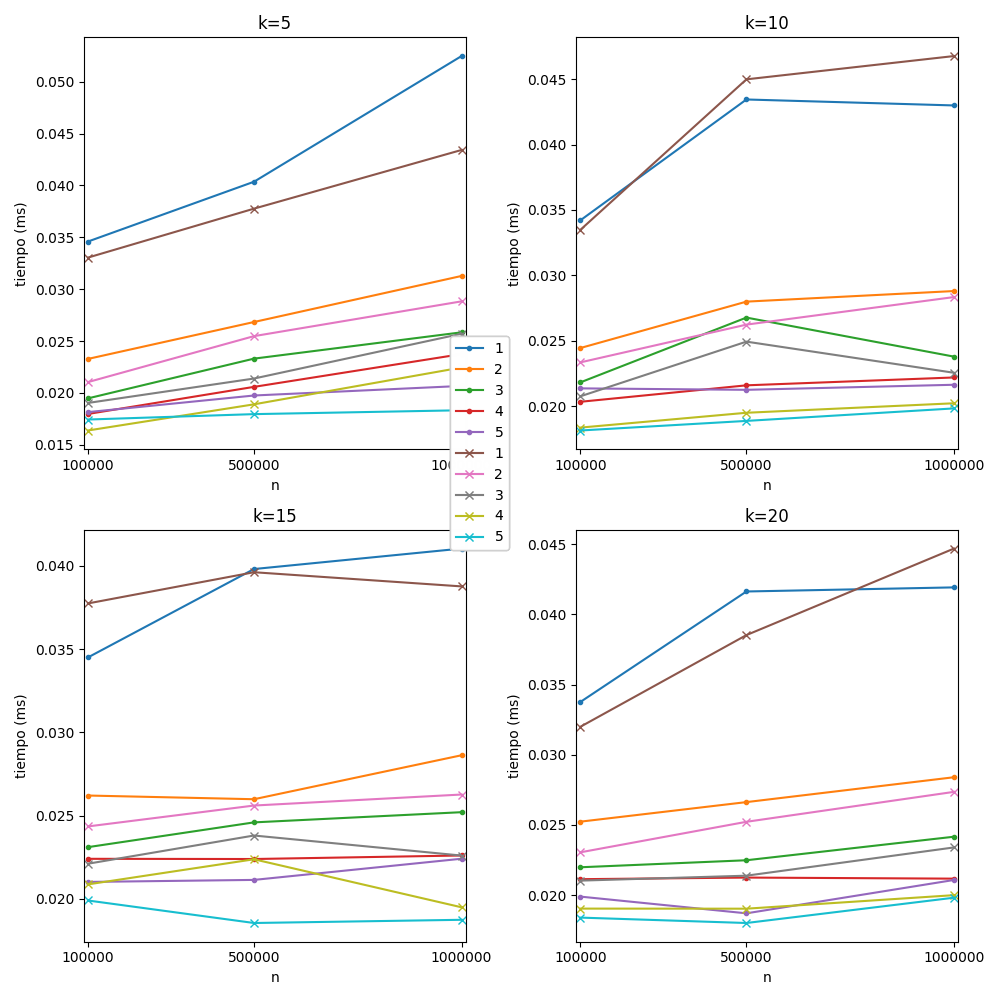
\includegraphics[width=.7\textwidth]{buscar_n}
  \caption{Tiempo de búsqueda (positiva y negativa)
    según n, para distintos valores de r y k.}
  \label{fig:buscar}
  \end{center}
\end{figure}

Esto se alinea con el desarrollo teórico, ya que \(r\) indica el factor de
ramificación, y cuanto mayor sea menos niveles debe recorrer hasta completar la
búsqueda.

Se observa una pequeña superioridad de las búsquedas negativas ante las positivas,
pero la diferencia no es significativa.

\begin{figure}
  \begin{center}
  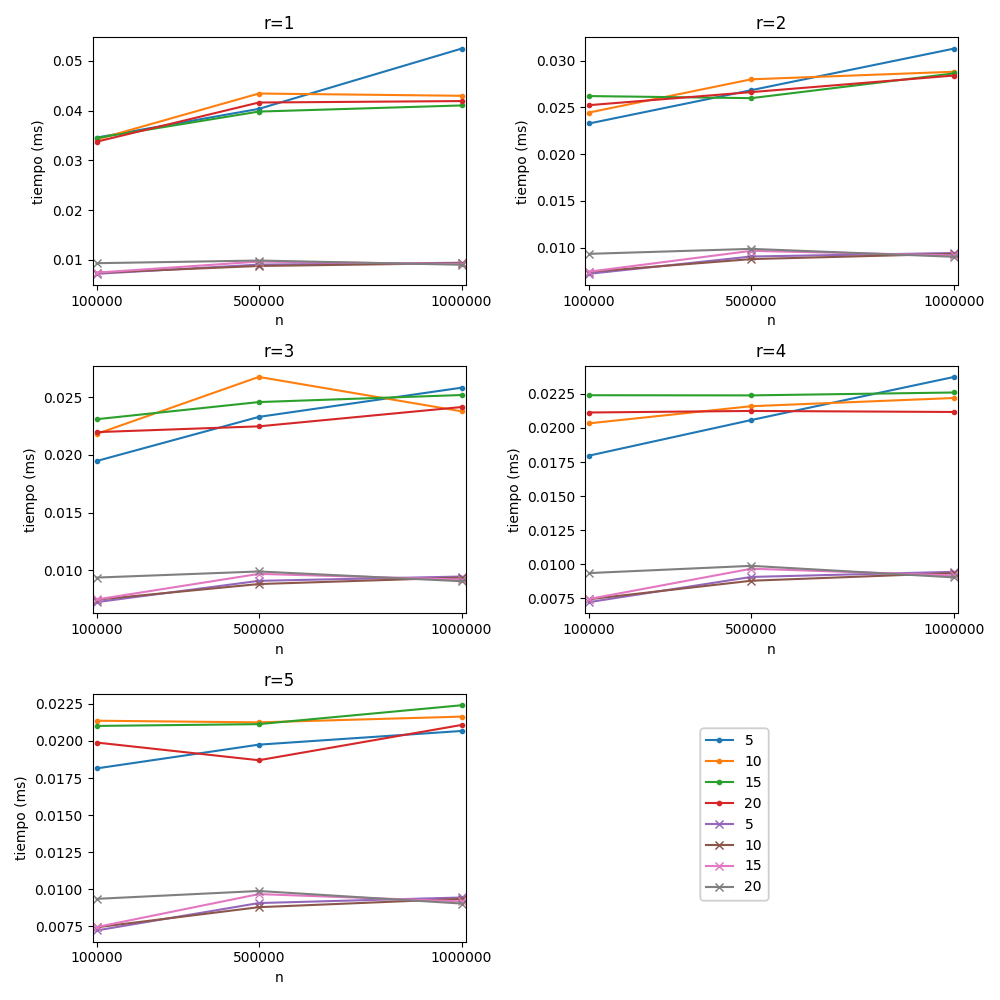
\includegraphics[width=.7\textwidth]{buscar_pos_kd_n}
  \caption{Tiempo de búsqueda (positiva)
    según n, para distintos valores de r y k, comparado con el arbol kd.}
  \label{fig:pos-kd}
  \end{center}
\end{figure}


\begin{figure}
  \begin{center}
  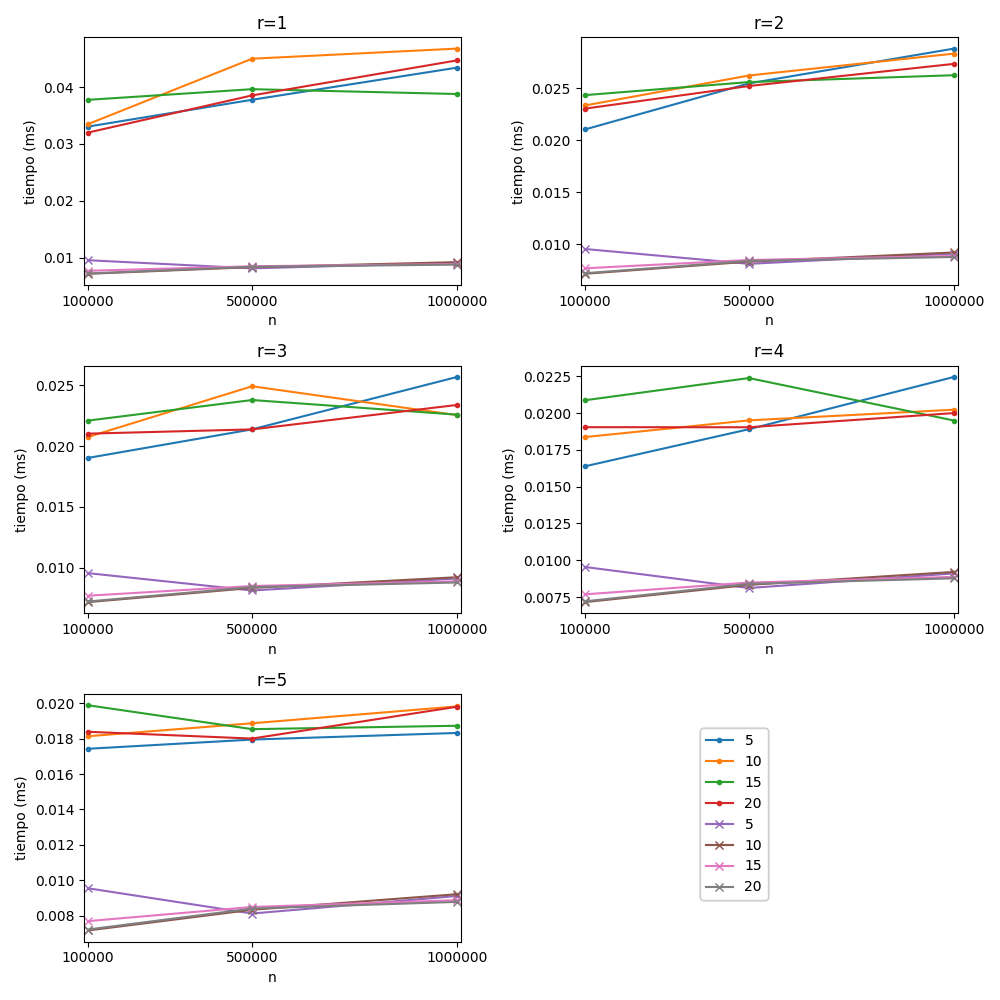
\includegraphics[width=.7\textwidth]{buscar_neg_kd_n}
  \caption{Tiempo de búsqueda (negativa)
    según n, para distintos valores de r y k, comparado con el arbol kd.}
  \label{fig:neg-kd}
  \end{center}
\end{figure}